\chapter{Advanced Model Recursions} \label{adv_models}


The surrogate and nested model constructs admit a wide variety of
multi-iterator, multi-model solution approaches.  For example,
optimization within optimization (for hierarchical multidisciplinary
optimization), uncertainty quantification within uncertainty
quantification (for interval-valued or second-order probability), uncertainty
quantification within optimization (for optimization under
uncertainty), and optimization within uncertainty quantification (for
uncertainty of optima) are all supported, with and without surrogate
model indirection.  Three important examples are highlighted:
second-order probability, optimization under uncertainty, and surrogate-based
uncertainty quantification.

\section{Mixed Aleatory-Epistemic UQ} \label{adv_models:mixed_uq}

Mixed UQ approaches employ nested models to embed one uncertainty
quantification (UQ) within another.  The outer level UQ is commonly
linked to epistemic uncertainties (also known as reducible
uncertainties) resulting from a lack of knowledge, and the inner UQ is
commonly linked to aleatory uncertainties (also known as irreducible
uncertainties) that are inherent in nature. The outer level generates
sets of realizations of the epistemic parameters, and each set of
these epistemic parameters in used within a separate inner loop
probabilistic analysis over the aleatory random variables.  In this
manner, ensembles of aleatory statistics are generated, one set for
each realization of the epistemic parameters.  %This ensemble is then
%interpreted in different ways according to the outer loop methodology
%that is employed.

In DAKOTA, we support interval-valued probability (IVP), second-order
probability (SOP), and Dempster-Shafer theory of evidence (DSTE)
approaches to mixed uncertainty.  These three approaches differ by how
they treat the epistemic variables in the outer loop: they are treated
as intervals in IVP, as subjective probability distributions in SOP,
and as belief structures in DSTE.  This set of techniques provides a
spectrum of assumed epistemic structure, from strongest assumptions in
SOP to weakest in IVP.

\subsection{Interval-valued probability (IVP)} \label{adv_models:mixed_uq:ivp}

In IVP (also known as probability bounds
analysis~\cite{Fer06,KaKiVeAj09,Aug07}), we employ an outer loop
of interval estimation in combination with an aleatory inner loop.
%These approaches can be considered to be a special case of imprecise
%probability theory.  
In interval analysis, it is assumed that nothing is known
about the uncertain input variables except that they lie within
certain intervals.  The problem of uncertainty propagation then
becomes an interval analysis problem: given inputs that are defined
within intervals, what is the corresponding interval on the outputs?
%Although interval analysis is conceptually simple, in practice it can
%be difficult to determine the more effective solution approach.  A direct
%approach is to use optimization to find the maximum and minimum values
%of the output measure of interest, which correspond to the upper and
%lower interval bounds on the output, respectively.  In practice, it
%may require a large number of function evaluations to determine these
%optima, especially if the simulation is very nonlinear with respect to
%the inputs, has a high number of inputs with interaction effects,
%exhibits discontinuities, etc.

%In IVP, we segregate the aleatory and epistemic variables and 
%perform nested iteration~\cite{helton_2009}.  
Starting from a specification of intervals and probability distributions 
on the inputs, %(as described in Section~\ref{sec:ssa:io}, 
the intervals may augment the probability distributions, insert into
the probability distributions, or some combination.  We generate an
ensemble of cumulative distribution functions (CDF) or Complementary
Cumulative Distribution Functions (CCDF), one CDF/CCDF result for each
aleatory analysis.  Plotting an entire ensemble of CDFs or CCDFs in a 
``horsetail'' plot allows one to visualize the upper and lower bounds 
on the family of distributions (see Figure~\ref{fig:horsetail}).
\begin{figure}[h!]% order of placement preference: here, top, bottom
 \begin{center}
 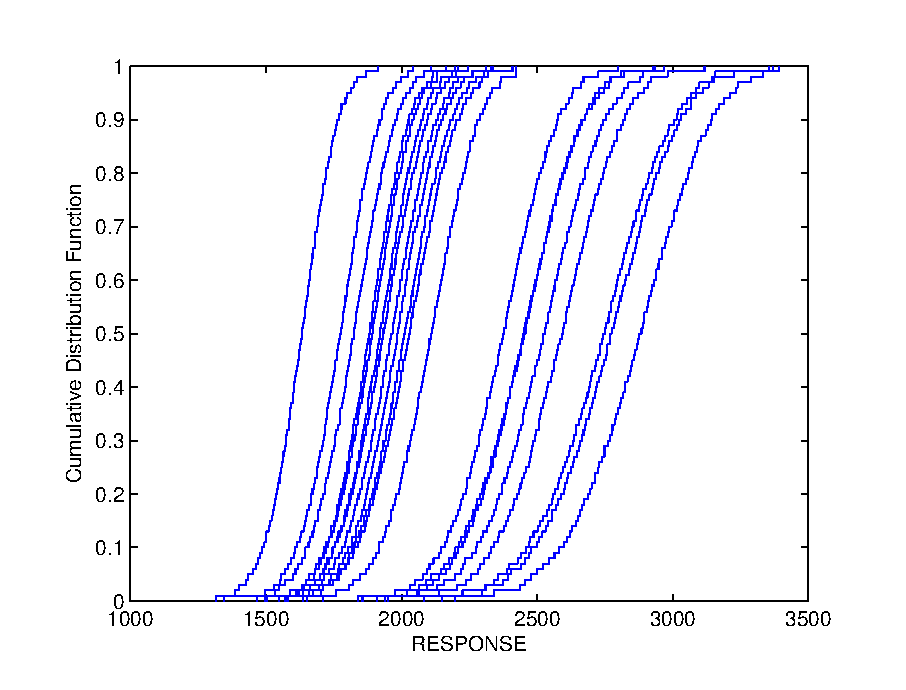
\includegraphics[width = 3.5in]{images/horsetail}
 \caption{Example CDF ensemble.  Commonly referred to as a ``horsetail'' plot.}
 \label{fig:horsetail}
 \end{center} 
\end{figure}
%However, nested iteration can be computationally expensive when it is
%implemented using two random sampling loops.  Consequently, when
%employing simulation-based models, the nested sampling must often be
%under-resolved, particularly at the epistemic outer loop, 
%resulting in an under-prediction of credible output ranges.  
Given that the ensemble stems from multiple
realizations of the epistemic uncertainties, the interpretation is
that each CDF/CCDF instance has no relative probability of occurrence,
only that each instance is possible.  For prescribed response levels
on the CDF/CCDF, an interval on the probability is computed based on
the bounds of the ensemble at that level, and vice versa for
prescribed probability levels.  This interval on a statistic is
interpreted simply as a possible range, where the statistic could take
any of the possible values in the range.

A sample input file is shown in
Figure~\ref{adv_models:2ndprob}, in which the outer epistemic level
variables are defined as intervals.  This file is
\texttt{dakota\_uq\_cantilever\_sop\_rel.in} in
\texttt{Dakota/examples/methods}.  Samples will be generated from
these intervals to select means for $X$ and $Y$ that are employed in
an inner level reliability analysis of the cantilever problem (see
Section~\ref{additional:cantilever}).
Figure~\ref{adv_models:2ndprob_res} shows excerpts from the resulting
output.  In this particular example, the outer loop generates 50
possible realizations of epistemic variables, which are then sent to
the inner loop to calculate statistics such as the mean weight, and
cumulative distribution function for the stress and displacement
reliability indices.  Thus, the outer loop has 50 possible values for
the mean weight but there is no distribution structure on these 50
samples.  So, only the minimum and maximum value are reported.
Similarly, the minimum and maximum values of the CCDF for the stress
and displacement reliability indices are reported.

When performing an epistemic analysis, response levels and 
probability levels should only be defined in the inner loop. 
For example, if one wants to generate an interval around possible 
CDFs or CCDFS, we suggest defining a number of probability levels 
in the inner loop (0.1, 0.2, 0.3, etc).  For each epistemic instance, 
these will be calculated during the inner loop and reported back to the 
outer loop.  In this way, there will be an ensemble of CDF percentiles 
(for example) and one will have interval bounds for each of these 
percentile levels defined.  Finally, although the epistemic variables are 
often values defining distribution parameters for the inner loop, 
they are not required to be: they can just be separate uncertain variables 
in the problem. 
\begin{figure}
  \centering
  \begin{bigbox}
    \begin{tiny}
      \verbatimtabinput[8]{dakota_uq_cantilever_sop_rel.in}
    \end{tiny}
  \end{bigbox}
  \caption{DAKOTA input file for the interval-valued probability example.}
  \label{adv_models:2ndprob}
\end{figure}

\begin{figure}
\centering
\begin{bigbox}
\begin{small}
\begin{verbatim}
Statistics based on 50 samples:

Min and Max values for each response function:
mean_wt:  Min = 9.5209117200e+00  Max = 9.5209117200e+00
ccdf_beta_s:  Min = 1.7627715524e+00  Max = 4.2949468386e+00
ccdf_beta_d:  Min = 2.0125192955e+00  Max = 3.9385559339e+00
\end{verbatim}
\end{small}
\end{bigbox}
\caption{Interval-valued statistics for cantilever beam reliability indices.}
\label{adv_models:2ndprob_res}
\end{figure}

As compared to aleatory quantities of interest (e.g., mean, variance,
probability) that must be integrated over a full probability domain,
we observe that the desired minima and maxima of the output ranges are
local point solutions in the epistemic parameter space, such that we
may employ directed optimization techniques to compute these extrema
and potentially avoid the cost of sampling the full epistemic space.
%resulting in more precise output bounds at lower cost.

In \texttt{dakota/test}, test input files such as
\texttt{dakota\_uq\_cantilever\_ivp\_exp.in} and\\
\texttt{dakota\_uq\_short\_column\_ivp\_exp.in} replace the outer loop
sampling with the local and global interval optimization methods
described in Section~\ref{uq:interval}.  In these cases, we no longer
generate horse tails and infer intervals, but rather compute the
desired intervals directly.


\subsection{Second-order probability (SOP)} \label{adv_models:mixed_uq:sop}

SOP is similar to IVP in its segregation of aleatory and epistemic
uncertainties and its use of nested iteration. However, rather than
modeling epistemic uncertainty with a single interval per variable and
computing interval-valued statistics, we instead employ subjective
probability distributions and compute epistemic statistics on the
aleatory statistics (for example, probabilities on probabilities --
the source of the ``second-order'' terminology~\cite{GoNg99}).  Now
the different hairs of the horsetail shown in
Figure~\ref{fig:horsetail} have a relative probability of occurrence
and stronger inferences may be drawn.  In particular, mean, 5$^{th}$
percentile, and 95$^{th}$ percentile probability values are a common
example. Second-order probability is sometimes referred to as
probability of frequency (PoF) analysis, referring to a probabilistic
interpretation of the epistemic variables and a frequency
interpretation of the aleatory variables.  The PoF terminology is used
in a recent National Academy of Sciences report on the Quantification
of Margins and Uncertainties (QMU)~\cite{NAS08}.

Rather than employing interval estimation techniques at the outer loop
in SOP, we can instead rely on the same probabilistic methods for
aleatory propagation employed for the inner loop.  In certain special
cases, expected values of expected values can be computed in closed
form (selected statistics for combined variable stochastic expansions,
refer to the DAKOTA Theory Manual~\cite{TheoMan}), without need for a
separate outer loop method.

The previous example in Figure~\ref{adv_models:2ndprob} can be
modified to define the epistemic outer loop using uniform variables
instead of interval variables (annotated test \texttt{\#1} in
\texttt{dakota/test/dakota\_uq\_cantilever\_sop\_rel.in}).  The process of
generating the epistemic values is essentially the same in both cases;
however, the interpretation of results is quite different.  In IVP,
each ``hair'' or individual CDF in the horsetail plot in
Figure~\ref{fig:horsetail} would be interpreted as a possible
realization of aleatory uncertainty conditional on a particular
epistemic sample realization.  The ensemble then indicates the
influence of the epistemic variables (e.g. by how widespread the
ensemble is).  However, if the outer loop variables are defined to be
uniformly distributed in SOP, then the outer loop results will be
reported as statistics (such as mean and standard deviation) and not
merely intervals.  It is important to emphasize that these outer level
output statistics are only meaningful to the extent that the outer
level input probability specifications are meaningful (i.e., to the
extent that the epistemic variables are known to be uniform).

In \texttt{dakota/test}, additional test input files such as
\texttt{dakota\_uq\_cantilever\_sop\_exp.in} and\\
\texttt{dakota\_uq\_short\_column\_sop\_exp.in} explore other outer/inner
loop probabilistic analysis combinations, particulary using stochastic
expansion methods .

\subsection{Dempster-Shafer Theory of Evidence} \label{adv_models:mixed_uq:dste}

In IVP, we estimate a single epistemic output interval for each
aleatory statistic.  This same nested analysis procedure may be
employed within the cell computations of a DSTE approach.  Instead of
a single interval, we now compute multiple output intervals, one for
each combination of the input basic probability assignments, in order
to define epistemic belief and plausibility functions on the aleatory
statistics computed in the inner loop.  While this can significantly
increase the computational requirements, belief and plausibility
functions provide a more finely resolved epistemic characterization
than a basic output interval.

The single-level DSTE approach for propagating epistemic uncertainties
is described in Section~\ref{uq:dempshaf} and in the DAKOTA Theory
Manual~\cite{TheoMan}.  Examples of nested DSTE for propagating mixed
uncertainties can be seen in \texttt{dakota/test} in the input file
\texttt{dakota\_uq\_ishigami\_dste\_exp.in}.


\section{Optimization Under Uncertainty (OUU)} \label{adv_models:ouu}

Optimization under uncertainty (OUU) approaches incorporate an
uncertainty quantification method within the optimization
process. This is often needed in engineering design problems when one
must include the effect of input parameter uncertainties on the
response functions of interest. A typical engineering example of OUU
would minimize the probability of failure of a structure for a set of
applied loads, where there is uncertainty in the loads and/or material
properties of the structural components.

In OUU, a nondeterministic method is used to evaluate the effect of
uncertain variable distributions on response functions of interest
(refer to Chapter~\ref{uq} for additional information on
nondeterministic analysis). Statistics on these response functions are
then included in the objective and constraint functions of an
optimization process.  Different UQ methods can have very different
features from an optimization perspective, leading to the tailoring of
optimization under uncertainty approaches to particular underlying UQ
methodologies.

If the UQ method is sampling based, then three approaches are
currently supported: nested OUU, surrogate-based OUU, and trust-region
surrogate-based OUU.  Additional details and computational results are
provided in~\cite{Eld02}.

Another class of OUU algorithms is called reliability-based design
optimization (RBDO).  RBDO methods are used to perform design
optimization accounting for reliability metrics.  The reliability
analysis capabilities described in Section~\ref{uq:reliability}
provide a rich foundation for exploring a variety of RBDO
formulations.  \cite{Eld05} investigated bi-level, fully-analytic
bi-level, and first-order sequential RBDO approaches employing
underlying first-order reliability assessments.
\cite{Eld06a} investigated fully-analytic bi-level and 
second-order sequential RBDO approaches employing underlying
second-order reliability assessments.  

When using stochastic expansions for UQ, analytic moments and
analytic design sensitivities can be exploited as described
in~\cite{Eld07}.  Several approaches for obtaining design
sensitivities of statistical metrics are discussed in 
Section~\ref{adv_models:ouu:sebdo}.

Finally, when employing epistemic methods for UQ, the set of
statistics available for use within optimization are interval-based.
Robustness metrics typically involve the width of the intervals, and
reliability metrics typically involve the worst case upper or lower
bound of the interval.

Each of these OUU methods is overviewed in the following sections.

\subsection{Nested OUU}\label{adv_models:ouu:nested}

In the case of a nested approach, the optimization loop is the outer
loop which seeks to optimize a nondeterministic quantity (e.g.,
minimize probability of failure). The uncertainty quantification (UQ)
inner loop evaluates this nondeterministic quantity (e.g., computes
the probability of failure) for each optimization function evaluation.
Figure~\ref{adv_models:figure08} depicts the nested OUU iteration where
$\mathit{\mathbf{d}}$ are the design variables, $\mathit{\mathbf{u}}$
are the uncertain variables characterized by probability
distributions, $\mathit{\mathbf{r_{u}(d,u)}}$ are the response
functions from the simulation, and $\mathit{\mathbf{s_{u}(d)}}$ are
the statistics generated from the uncertainty quantification on these
response functions.

\begin{figure}
  \centering
  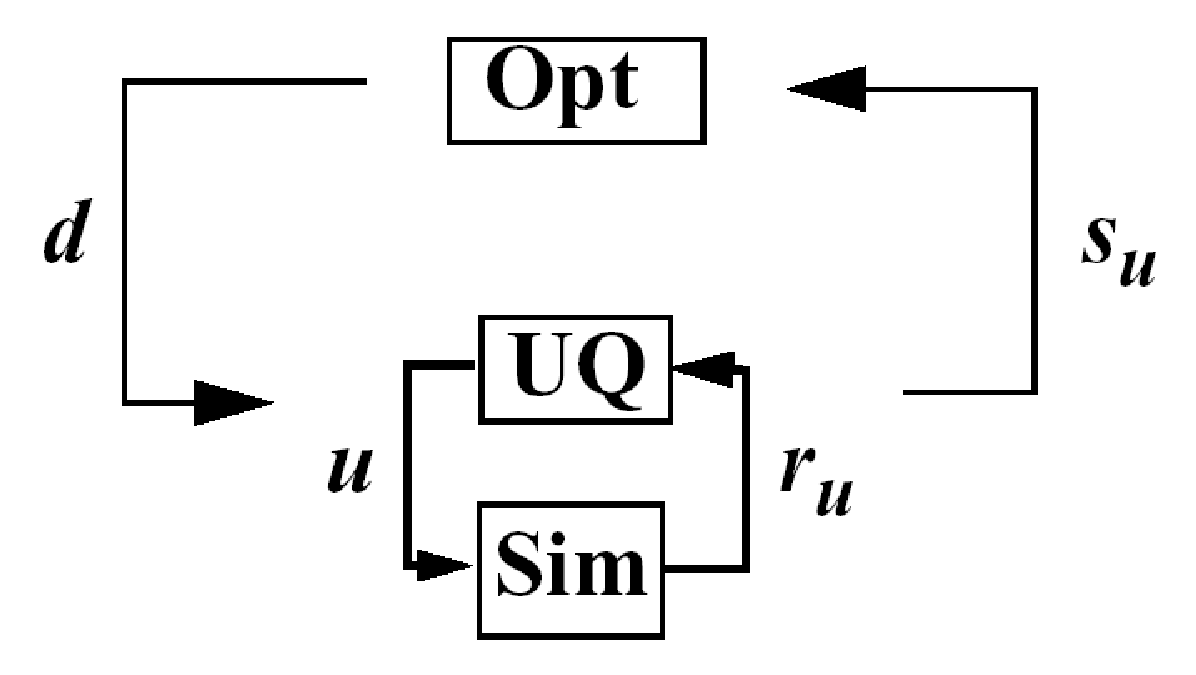
\includegraphics[scale=0.33]{images/nested_ouu}
  \caption{Formulation 1: Nested OUU.}
  \label{adv_models:figure08}
\end{figure}

Figure~\ref{adv_models:figure09} shows a DAKOTA input file for a nested
OUU example problem that is based on the textbook test problem. This
input file is named \texttt{dakota\_ouu1\_tb.in} in the
\texttt{dakota/test} directory.  In this example, the objective
function contains two probability of failure estimates, and an
inequality constraint contains another probability of failure
estimate. For this example, failure is defined to occur when one of
the textbook response functions exceeds its threshold value. The
strategy keyword block at the top of the input file identifies this as
an OUU problem. The strategy keyword block is followed by the
optimization specification, consisting of the optimization method, the
continuous design variables, and the response quantities that will be
used by the optimizer. The mapping matrices used for incorporating UQ
statistics into the optimization response data are described in the
DAKOTA Reference Manual~\cite{RefMan}. The uncertainty quantification
specification includes the UQ method, the uncertain variable
probability distributions, the interface to the simulation code, and
the UQ response attributes. As with other complex DAKOTA input files,
the identification tags given in each keyword block can be used to
follow the relationships among the different keyword blocks.

\begin{figure}
  \centering
  \begin{bigbox}
    \begin{tiny}
      \verbatimtabinput[8]{dakota_ouu1_tb.in}
    \end{tiny}
  \end{bigbox}
  \caption{DAKOTA input file for the nested OUU example.}
  \label{adv_models:figure09}
\end{figure}

Latin hypercube sampling is used as the UQ method in this example
problem. Thus, each evaluation of the response functions by the
optimizer entails 50 Latin hypercube samples. In general, nested OUU
studies can easily generate several thousand function evaluations and
gradient-based optimizers may not perform well due to noisy or
insensitive statistics resulting from under-resolved sampling. These
observations motivate the use of surrogate-based approaches to OUU.

Other nested OUU examples in the \texttt{dakota/test} directory
include \texttt{dakota\_ouu1\_tbch.in}, which adds an additional
interface for including deterministic data in the textbook OUU
problem, and\\ \texttt{dakota\_ouu1\_cantilever.in}, which solves the
cantilever OUU problem (see Section~\ref{additional:cantilever}) with
a nested approach. For each of these files, the ``\texttt{1}''
identifies formulation 1, which is short-hand for the nested approach.

% TO DO: combine with TR-SBOUU discussion?
\subsection{Surrogate-Based OUU (SBOUU)}\label{adv_models:ouu:sb}

Surrogate-based optimization under uncertainty strategies can be
effective in reducing the expense of OUU studies. Possible
formulations include use of a surrogate model at the optimization
level, at the uncertainty quantification level, or at both levels.
These surrogate models encompass both data fit surrogates (at the
optimization or UQ level) and model hierarchy surrogates (at the UQ
level only). Figure~\ref{adv_models:figure10} depicts the different
surrogate-based formulations where $\mathbf{\hat{r}_{u}}$ and
$\mathbf{\hat{s}_{u}}$ are approximate response functions and
approximate response statistics, respectively, generated from the
surrogate models.

\begin{figure}
  \centering
  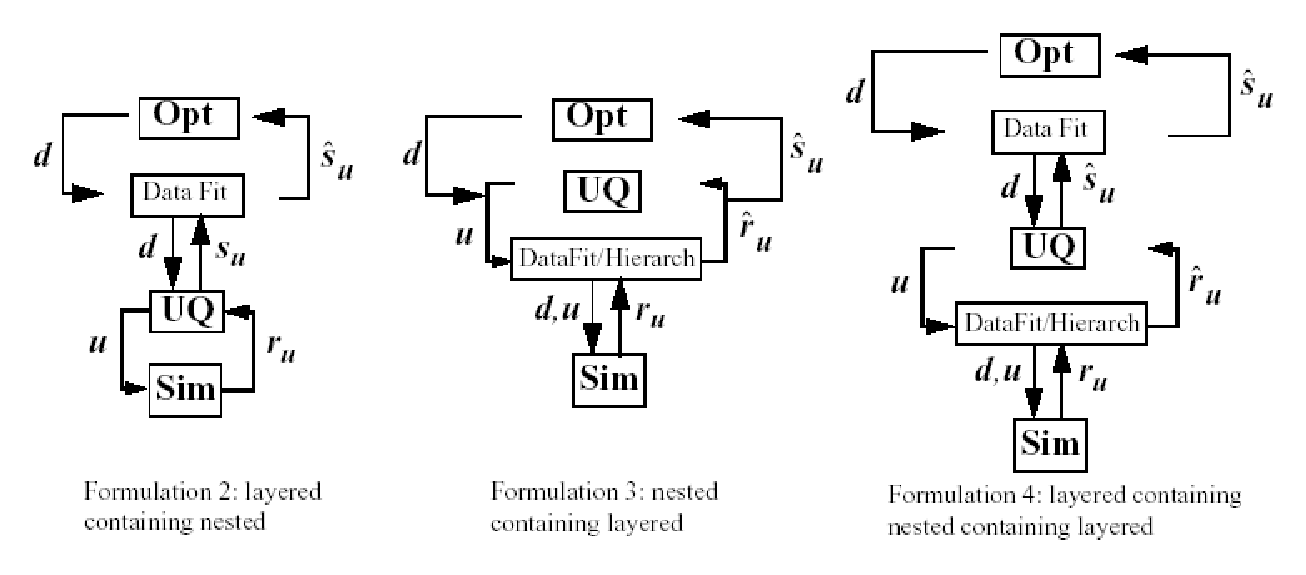
\includegraphics[scale=0.65]{images/sbouu}
  \caption{Formulations 2, 3, and 4 for Surrogate-based OUU.}
  \label{adv_models:figure10}
\end{figure}

SBOUU examples in the \texttt{dakota/test} directory include
\texttt{dakota\_sbouu2\_tbch.in},\\ \texttt{dakota\_sbouu3\_tbch.in},
and \texttt{dakota\_sbouu4\_tbch.in}, which solve the textbook OUU
problem, and \texttt{dakota\_sbouu2\_cantilever.in},
\texttt{dakota\_sbouu3\_cantilever.in}, and\\
\texttt{dakota\_sbouu4\_cantilever.in}, which solve the cantilever OUU
problem (see Section~\ref{additional:cantilever}). For each of these
files, the ``\texttt{2},'' ``\texttt{3},'' and ``\texttt{4}'' identify
formulations 2, 3, and 4, which are short-hand for the ``layered
containing nested,'' ``nested containing layered,'' and ``layered
containing nested containing layered'' surrogate-based formulations,
respectively. In general, the use of surrogates greatly reduces the
computational expense of these OUU study. However, without restricting
and verifying the steps in the approximate optimization cycles,
weaknesses in the data fits can be exploited and poor solutions may be
obtained. The need to maintain accuracy of results leads to the use of
trust-region surrogate-based approaches.

\subsection{Trust-Region Surrogate-Based OUU (TR-SBOUU)}\label{adv_models:ouu:trsb}

The TR-SBOUU approach applies the trust region logic of deterministic
SBO (see Section~\ref{sbm:sblm}) to SBOUU. Trust-region verifications
are applicable when surrogates are used at the optimization level,
i.e., formulations 2 and 4. As a result of periodic verifications and
surrogate rebuilds, these techniques are more expensive than SBOUU;
however they are more reliable in that they maintain the accuracy of
results. Relative to nested OUU (formulation 1), TR-SBOUU tends to be
less expensive and less sensitive to initial seed and starting point.

TR-SBOUU examples in the \texttt{dakota/test} directory include
\texttt{dakota\_trsbouu2\_tbch.in} and\\
\texttt{dakota\_trsbouu4\_tbch.in}, which solve the textbook OUU
problem, and\\ \texttt{dakota\_trsbouu2\_cantilever.in} and
\texttt{dakota\_trsbouu4\_cantilever.in}, which solve the cantilever
OUU problem (see Section~\ref{additional:cantilever}).

Computational results for several example problems are available
in~\cite{Eld02}.

\subsection{RBDO} \label{adv_models:ouu:rbdo}

Bi-level and sequential approaches to reliability-based design
optimization (RBDO) and their associated sensitivity analysis
requirements are described in the Optimization Under Uncertainty
chapter of the DAKOTA Theory Manual~\cite{TheoMan}.

A number of bi-level RBDO examples are provided in \texttt{dakota/test}.
The \texttt{dakota\_rbdo\_cantilever.in},
\texttt{dakota\_rbdo\_short\_column.in}, and
\texttt{dakota\_rbdo\_steel\_column.in} input files solve the
cantilever (see Section~\ref{additional:cantilever}), short column
(see Section~\ref{additional:short_column}), and steel column (see
Section~\ref{additional:steel_column}) OUU problems using a bi-level
RBDO approach employing numerical design gradients.  The 
\texttt{dakota\_rbdo\_cantilever\_analytic.in} and
\texttt{dakota\_rbdo\_short\_column\_analytic.in} input files solve
the cantilever and short column OUU problems using a bi-level RBDO
approach with analytic design gradients and first-order limit state
approximations.  The \texttt{dakota\_rbdo\_cantilever\_analytic2.in},
\texttt{dakota\_rbdo\_short\_column\_analytic2.in}, and
\texttt{dakota\_rbdo\_steel\_column\_analytic2.in} input files also
employ analytic design gradients, but are extended to employ
second-order limit state approximations and integrations.

Sequential RBDO examples are also provided in \texttt{dakota/test}.  
The \texttt{dakota\_rbdo\_cantilever\_trsb.in} and
\texttt{dakota\_rbdo\_short\_column\_trsb.in} input files solve 
the cantilever and short column OUU problems using a first-order
sequential RBDO approach with analytic design gradients and
first-order limit state approximations.  The
\texttt{dakota\_rbdo\_cantilever\_trsb2.in},
\texttt{dakota\_rbdo\_short\_column\_trsb2.in}, and 
\texttt{dakota\_rbdo\_steel\_column\_trsb2.in} input files 
utilize second-order sequential RBDO approaches that employ
second-order limit state approximations and integrations (from
analytic limit state Hessians with respect to the uncertain variables)
and quasi-Newton approximations to the reliability metric Hessians
with respect to design variables.

\subsection{Stochastic Expansion-Based Design Optimization} \label{adv_models:ouu:sebdo}

For stochastic expansion-based approaches to optimization under
uncertainty, bi-level, sequential, and multifidelity approaches and
their associated sensitivity analysis requirements are described in
the Optimization Under Uncertainty chapter of the DAKOTA Theory
Manual~\cite{TheoMan}.

In \texttt{dakota/test}, the \texttt{dakota\_pcbdo\_cantilever.in},
\texttt{dakota\_pcbdo\_rosenbrock.in},\\
\texttt{dakota\_pcbdo\_short\_column.in}, and
\texttt{dakota\_pcbdo\_steel\_column.in} input files solve cantilever
(see Section~\ref{additional:cantilever}), Rosenbrock, short column
(see Section~\ref{additional:short_column}), and steel column (see
Section~\ref{additional:steel_column}) OUU problems using a bi-level
polynomial chaos-based approach, where the statistical design metrics
are reliability indices based on moment projection (see Mean Value
section in Reliability Methods Chapter of DAKOTA Theory
Manual~\cite{TheoMan}).  The test matrix in the former three input
files evaluate design gradients of these reliability indices using
several different approaches: analytic design gradients based on a PCE
formed over only over the random variables, analytic design gradients
based on a PCE formed over all variables, numerical design gradients
based on a PCE formed only over the random variables, and numerical
design gradients based on a PCE formed over all variables.  In the
cases where the expansion is formed over all variables, only a single
PCE construction is required for the complete PCBDO process, whereas
the expansions only over the random variables must be recomputed for
each change in design variables.  Sensitivities for ``augmented''
design variables (which are separate from and augment the random
variables) may be handled using either analytic approach; however,
sensitivities for ``inserted'' design variables (which define
distribution parameters for the random variables) must be 
%handled using Eqs.~\ref{eq:dmuR_ds_xi_pce}-\ref{eq:dsigR_ds_xi_pce} 
%where $\frac{dR}{ds}$ is calculated as $\frac{dR}{dx} \frac{dx}{ds}$.
computed using $\frac{dR}{dx} \frac{dx}{ds}$ (refer to Stochastic
Sensitivity Analysis section in Optimization Under Uncertainty chapter
of DAKOTA Theory Manual~\cite{TheoMan}).  Additional test input files
include:
\begin{itemize}
\item \texttt{dakota\_scbdo\_cantilever.in}, 
\texttt{dakota\_scbdo\_rosenbrock.in}, \\
\texttt{dakota\_scbdo\_short\_column.in}, and
\texttt{dakota\_scbdo\_steel\_column.in} input files solve 
cantilever, Rosenbrock, short column, and steel column OUU problems
using a bi-level stochastic collocation-based approach.

\item \texttt{dakota\_pcbdo\_cantilever\_trsb.in},
\texttt{dakota\_pcbdo\_rosenbrock\_trsb.in}, \\
\texttt{dakota\_pcbdo\_short\_column\_trsb.in}, 
\texttt{dakota\_pcbdo\_steel\_column\_trsb.in},\\
\texttt{dakota\_scbdo\_cantilever\_trsb.in}, 
\texttt{dakota\_scbdo\_rosenbrock\_trsb.in}, \\
\texttt{dakota\_scbdo\_short\_column\_trsb.in}, and
\texttt{dakota\_scbdo\_steel\_column\_trsb.in} input files solve 
cantilever, Rosenbrock, short column, and steel column OUU problems
using sequential polynomial chaos-based and stochastic
collocation-based approaches.

\item \texttt{dakota\_pcbdo\_cantilever\_mf.in},
\texttt{dakota\_pcbdo\_rosenbrock\_mf.in}, \\
\texttt{dakota\_pcbdo\_short\_column\_mf.in}, 
\texttt{dakota\_scbdo\_cantilever\_mf.in}, \\
\texttt{dakota\_scbdo\_rosenbrock\_mf.in}, and
\texttt{dakota\_scbdo\_short\_column\_mf.in} input files solve 
cantilever, Rosenbrock, and short column OUU problems
using multifidelity polynomial chaos-based and stochastic
collocation-based approaches.
\end{itemize}


\subsection{Epistemic OUU} \label{adv_models:ouu:epistemic}

An emerging capability is optimization under epistemic uncertainty.
As described in the Nested Model section of the Reference
Manual~\cite{RefMan}, epistemic and mixed aleatory/epistemic
uncertainty quantification methods generate lower and upper interval
bounds for all requested response, probability, reliability, and
generalized reliability level mappings.  Design for robustness in the
presence of epistemic uncertainty could simply involve minimizing the
range of these intervals (subtracting lower from upper using the
nested model response mappings), and design for reliability in the
presence of epistemic uncertainty could involve controlling the worst
case upper or lower bound of the interval.

We now have the capability to perform epistemic analysis by 
using interval optimization on the ``outer loop'' to calculate bounding 
statistics of the aleatory uncertainty on the ``inner loop.''  
Preliminary studies~\cite{Eld09b} have shown this approach is more efficient 
and accurate than nested sampling (which was described in 
Section~\ref{adv_models:mixed_uq:sop}).  This approach uses 
an efficient global optimization method for the outer loop and 
stochastic expansion methods (e.g. polynomial chaos or stochastic 
collocation on the inner loop).  The interval optimization is described in 
Section~\ref{uq:interval}.  Example input files demonstrating 
the use of interval estimation for epistemic analysis, 
specifically in epistemic-aleatory nesting, are: 
\texttt{dakota\_uq\_cantilever\_sop\_exp.in}, and
\texttt{dakota\_short\_column\_sop\_exp.in}. 

\section{Surrogate-Based Uncertainty Quantification} \label{adv_models:sbuq}

Many uncertainty quantification (UQ) methods are computationally costly. 
For example, sampling often requires many function evaluations to obtain 
accurate estimates of moments or percentile values of an output distribution.  
One approach to overcome the computational cost of sampling is to 
evaluate the true function (e.g. run the analysis driver) on a fixed, small
set of samples, use these sample evaluations to 
create a response surface approximation (e.g. a surrogate model or meta-model)
of the underlying ``true'' function, then perform random sampling (using 
thousands or millions of samples) on the approximation to obtain estimates 
of the mean, variance, and percentiles of the response. 

This approach, called ``surrogate-based uncertainty quantification'' 
is easy to do in DAKOTA, and one can set up input files to compare the 
results using no approximation (e.g. determine the mean, variance, and 
percentiles of the output directly based on the initial sample values) 
with the results obtained by sampling a variety of surrogate approximations.  
Example input files of a standard UQ analysis based on sampling alone vs. 
sampling a surrogate are shown in the \texttt{dakota\_uq\_sampling.in} and 
\texttt{dakota\_surr\_uq.in} in the \texttt{Dakota/examples/methods}
directory. 

Note that one must exercise some caution when using surrogate-based methods 
for uncertainty quantification. In general, there is not a single, 
straightforward approach to incorporate the error of the surrogate fit 
into the uncertainty estimates of the output produced by sampling the surrogate.
Two references which discuss some of the related 
issues are~\cite{Giu06} and~\cite{Swi06}. The first reference shows that 
statistics of a response based on a surrogate model were less accurate, and 
sometimes biased, for surrogates constructed on very small sample sizes.  
In many cases, however,~\cite{Giu06} shows that surrogate-based UQ performs 
well and sometimes generates more accurate estimates of statistical
quantities on the output.  The second reference goes into more detail 
about the interaction between sample type and response surface type (e.g., 
are some response surfaces more accurate when constructed on a particular 
sample type such as LHS vs. an orthogonal array?) In general, there is not 
a strong dependence of the surrogate performance with respect to sample type, 
but some sample types perform better with respect to some metrics and not 
others (for example, a Hammersley sample may do well at lowering root mean 
square error of the surrogate fit but perform poorly at lowering the maximum 
absolute deviation of the error).  Much of this work is empirical and 
application dependent.  If you choose to use surrogates in uncertainty 
quantification, we strongly recommend trying a variety of surrogates 
and examining diagnostic goodness-of-fit metrics. 
